% !TeX program = lualatex
% !TeX root = luaking.tex
% !TeX encoding = UTF-8
% !TeX spellcheck = cs_CZ
%---------------------------------------------------------------------------------------------------
% file ces1ch01.tex
%---------------------------------------------------------------------------------------------------
%============ Kapitola: Číslicové signály a systémy ================================================
\setchaptertoc
\chapter{Číslicové signály a systémy}\label{ces:IchapI}
    Při vymezování pojmu číslicový signál a číslicový systém vyjdeme z intuitivního chápání pojmů
    \emph{analogový signál} a \emph{analogový systém}, se kterým jsme se již seznámili v kapitole
    \ref{tky:IchII} v partii \ref{part:TKY}. 
    
    Analogovým signálem, přesněji řečeno \emph{signálem spojitým v čase}, budeme chápat reálnou
    funkci jedné reálné proměnné (ve většině případů bude nezávislou proměnnou čas). Systém schopný
    zpracovávat analogové signály budeme označovat jako analogový systém.

    Signál diskrétní v čase a nekvantovaný v úrovni, který získáme diskretizací analogového signálu,
    označujeme jako \emph{diskrétní signál}. Systémy pracující s tímto typem signálu jsou systémy s
    diskrétním časem - \emph{diskrétní systémy}. Přílady takových systémů jsou např. soustavy s
    přenosem náboje (CCD) nebo filtry se spínanými kapacitory (SC).

    Signál diskétní v čase a kvantovaný v úrovni budeme nazývat \textbf{číslicový signál} nebo
    \textbf{posloupnost}. Systémy pracující s tímto typem signálů nazýváme \emph{číslicové systémy}.
    Příkladem těchto systémů jsou např. CD/DVD přehrávače, syntezátory řeči, apod.
    (\cite[s.~1]{Davidek1996}).
    
  \section{Číslicové signály - posloupnosti}\label{ces:IchapIsecI}
    Číslicové signály (matematicky posloupnosti čísel) jsou v literatuře označovány symboly \(x_n\),
    \(x(n)\), nebo \(x[nT]\), kde \(n\) je celé číslo a označuje pořadí prvku v
    posloupnosti\footnote{Takto zavedené označení je nejednoznačné, neboť nerozlišuje mezi celou
    posloupností a jejím jediným prvkem. Posloupnost by měla být správně označena např. symbolem
    \(x[n]\), zatímco symbol \(x[n]\) by měl být vyhrazen pro její jeden prvek. Nicméně uvedené
    značení je všeobecně používáno.} Poslední uvedený symbol \(x[nT]\) zdůrazňuje souvislost
    číslicového signálu se signálem spojitým v čase(analogovým signálem), ze kterého vznikl
    vzorkováním a kvantováním. Symbol \(T\) označuje použitý \emph{vzorkovací krok}. Jeho převrácená
    hodnota je rovna \emph{vzorkovací frekvenci} \(f_s=\frac{1}{T}\).
    
    Grafická reprezentace číslicových signálů bývá buď ve \uv{spojité} formě (viz. obr
    \ref{ces:fig050}), nebo v \uv{diskrétní formě} (viz. obr. \ref{ces:fig051}).

    \luagraphic[1]{ces_fig050.png}{Spojitá grafická reprezentace číslicových signálů - konkrétně
      řečového signálu pomocí příkazu \lstinline[style=luaMatlabText]!plot(x)!, kde vektor \(x\)
      obsahuje vzorky signálu (\cite[s.~2]{Davidek1996}).}{ces:fig050}
  
    \luagraphic[1]{ces_fig051.png}{Diskrétní grafická reprezentace číslicových signálů - konkrétně
      je znázorněna část průbehu z předchozího obrázku pomocí příkazu
      \lstinline[style=luaMatlabText]!stem(x)! (\cite[s.~2]{Davidek1996}).}{ces:fig051}

    Pomocí zavedených pojů nyní můžeme zpřesnit vymezení číslicového systému. Systémy, které pracují
    s číslicovými signály (posloupnostmi) se nazývají \textbf{číslicové systémy}. Číslicovým
    systémem, tak jak jej v dalším textu budme používat, rozumíme \uv{černou skříňku}, která na
    vstupní posloupnost (signál) \(x[n]\) reaguje výstupní posloupností (signálem) \(y[n]\) (viz.
    \ref{ces:fig049}). Zajímá nás tedy popis systému pomocí vstupních a výstupných signálů, jejichž
    hodnoty budeme považovat za reálné. Nebudeme používat stavový ani maticový popis systému.
    Zaměříme se na systémy s \emph{jedním vstupem a jedním výstupem a reálnými parametry
    (koeficienty)}.
    
    \luagraphic[1]{ces_fig049.pdf}{Symbol číslicového systému se vstupním a výstupním
    signálem. (\cite[s.~2]{Davidek1996})}{ces:fig049}

  \section{Základní typy posloupností}\label{ces:IchapIsecII}
    Nyní si stručně popíšeme základní typy číslicových signálů, jejich význam a použití

    \subsection{Jednotkový impuls}
      Prvním z těchto signálů je \textbf{jednotkový impuls}
      \begin{equation}\label{ces:eq001}
        \delta[n]=
        \begin{cases} 
            1, &  n = 0, \\
             0, &  n \neq 0,
        \end{cases}
      \end{equation}
      který je zobrazen na obr. \ref{ces:fig051}. Je-li přiveden na vstup číslicové soustavy,
      objeví se na jejím výstupu \emph{impulsová odezva}. Tento signál je obdobou Diracova
      impulsu používaného v analové oblasti, i když fyzikálně se jedná o zcela odlišné
      signály. Rovněž matematická složitost definice obou impulsu je rozdílná. Použití
      jednotkového impulsu definovaného rovnicí \ref{ces:eq001} je velmi snadn0 a umo6=nuje
      realizovat výpočet impulsové odezvy libovolného systému jednoduchým způsobem
            
    \begin{itemize}
      \item \textbf{Jednotkový skok}
            \begin{equation}\label{ces:eq002}
              u[n]=
              \begin{cases} 
                 1, &  n \geq 0, \\
                 0, &  n < 0,
              \end{cases}
            \end{equation}
      \item \textbf{Reálná exponenciální posloupnost}
            \begin{equation}\label{SAS:eq_exp}
              x[n] = A\alpha^n, n\geq0,
            \end{equation}
      \item \textbf{Chirp signál}
            \begin{equation}\label{SAS:eq_chirp}
              x[n] = sin\left(\frac{\pi f_{max}n^2}{(N-1)f_s}\right),
            \end{equation}
            kde $f_{max}$ je maximální požadovaný kmitočet, který musí být menší než polovina
            vzorkovacího kmitočtu $f_{max}<\frac{f_s}{2}$ a $N$ je celkový počet vzorků.
      \item \textbf{Pseudonáhodná posloupnost} je posloupnost, která nahrazuje ideální bílý šum.
            Tuto posloupnost lze generovat různými algoritmy, které zaručují velmi dlouhou
            periodicitu generované posloupnosti. Má-li tato posloupnost aproximovat bílý šum, musí
            co nejlépe splňovat požadavek nekorelovanosti sousedních vzorků (tedy konstantní
            spektrální výkonové hustoty) a nulové střední hodnoty. Často je požadován i jednotkový
            rozptyl.
            \begin{figure}[ht!]
             \centering
             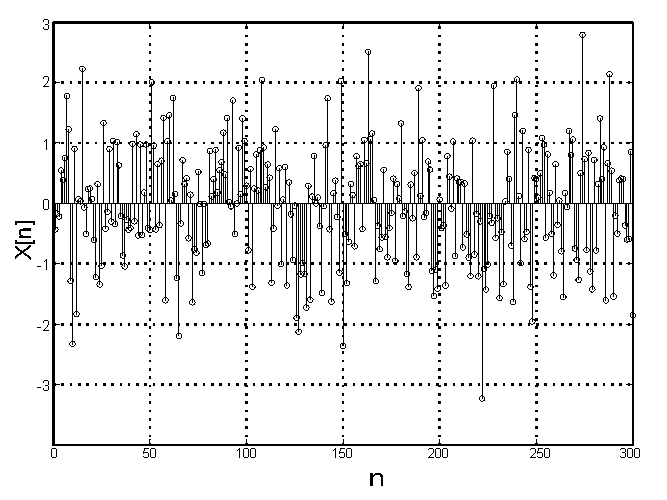
\includegraphics[width=1\linewidth]{ces_fig046.pdf}
             \caption[Příklad pseudonáhodné posloupnosti]{Příklad pseudonáhodné posloupnosti
                      generované pomocí funkce \texttt{randn(1, 300)} v MATLABu}
             \label{ces:fig046}
         \end{figure}
    \end{itemize}
    %---------------------------------------------------------------
    % !TeX spellcheck = cs_CZ
\begin{mdframed}[style=mdexam]
\begin{example}
  Generujte signál s lineárně rostoucím kmitočtem "\texttt{chirp signál}", maximální kmitočet
  $f_{max} = 20 Hz$, amplituda $A = 1$, vzorkovaný kmitočtem $f_s = 64 Hz$.

  {\centering
  \captionsetup{type=figure}
   \subcaptionbox{Spojitá forma   \label{mai:fig047a}}{\luafigure[1]{ces_fig047a.pdf}}              \newline
   \subcaptionbox{Diskrétní forma \label{mai:fig047b}}{\luafigure[1]{ces_fig047b.pdf}}
   \captionof{figure}{Chirp signál: Signál s lineárně rostoucím kmitočtem s maximální
    frekvencí 20 Hz vzorkovaný 254 Hz. Grafická reprezentace číslicových signálů bývá buď ve spojité
    formě (a) nebo v diskrétní formě (b) 
  \label{ces:fig047}}
\par}
\end{example}

  %---------------------------------------------------------------
  \lstinputlisting[%
    style=luaMatlabStyle,
    caption={\texttt{gen\_chirp\_signal.m}. Generuje chirp signál}
    ]{../src/CES/matlab/gen_chirp_signal.m}
  %--------------------------------------------------------------- 
\end{mdframed}
    %---------------------------------------------------------------
  \section{Generování jednoduchých signálů a jejich zobrazení v MATLABu}

  \section{Základní operace s posloupnosti}
    V dalším textu budeme používat tři základní lineární operace zobrazené na \ref{tky:fig_007}:
    \begin{itemize}
      \item \texttt{součin} signálu $x[n]$ a reálné konstanty $b$:
            $$w[n]=bx[n], n = 0,1,2, \ldots$$ Tato operace je v praxi realizována násobičkou a je
            zdrojem numerických chyb, tedy kvantizačního šumu, který produkují číslicová zařízení.
      \item \texttt{součet} signálu $x[n]$ a signálu $y[n]$:
            $$v[n]=x[n]+y[n], n = 0,1,2, \ldots$$ Tuto operaci provádí sčítačka. Při neošetření může
            tato operace generovat hrubé chyby.
      \item \texttt{zpoždění} signálu $x[n]$ o $k$ vzorkovacích kroků:  
            $$y[n]=x[n-k], n = 0,1,2, \ldots, n = 1,2, \ldots, M $$  Hodnoty $x[-k], k = 1, 2,
            \ldots, M$ se nazývají \emph{počáteční podmínky}. V digitálních implementací provádíme
            operaci zpoždění paměťového registru pro každou jednotku požadovaného zpoždění $z^{-1}$.
    \end{itemize}

    \begin{figure}[ht!]
      \centering
      \subcaptionbox{\label{tky:fig_007a}}{\luafigure[0.45]{ces_fig048a.pdf}}  
      \subcaptionbox{\label{tky:fig_007b}}{\luafigure[0.45]{ces_fig048b.pdf}}  \newline
      \subcaptionbox{\label{tky:fig_007c}}{\luafigure[0.45]{ces_fig048c.pdf}}
      \caption[Základní operace]{Symboly základních operací \cite[s.~7]{Sovka2002}} 
      \label{ces:fig048}
    \end{figure}